\documentclass[conference]{IEEEtran}
\IEEEoverridecommandlockouts
\usepackage{cite}
\usepackage{amsmath,amssymb,amsfonts}
\usepackage{algorithmic}
\usepackage{graphicx}
\usepackage{textcomp}
\usepackage{xcolor}
\usepackage{hyperref}
\usepackage{url}
\usepackage{subfigure}
\def\UrlBreaks{\do\A\do\B\do\C\do\D\do\E\do\F\do\G\do\H\do\I\do\J
\do\K\do\L\do\M\do\N\do\O\do\P\do\Q\do\R\do\S\do\T\do\U\do\V
\do\W\do\X\do\Y\do\Z\do\[\do\\\do\]\do\^\do\_\do\`\do\a\do\b
\do\c\do\d\do\e\do\f\do\g\do\h\do\i\do\j\do\k\do\l\do\m\do\n
\do\o\do\p\do\q\do\r\do\s\do\t\do\u\do\v\do\w\do\x\do\y\do\z
\do\.\do\@\do\\\do\/\do\!\do\_\do\|\do\;\do\>\do\]\do\)\do\,
\do\?\do\'\do+\do\=\do\#} 
\def\BibTeX{{\rm B\kern-.05em{\sc i\kern-.025em b}\kern-.08em
    T\kern-.1667em\lower.7ex\hbox{E}\kern-.125emX}}
\begin{document}

\title{High-Performance scRNA-seq Data Processing with Low-Redundancy Disk Access}

\author{\IEEEauthorblockN{Yu Liu}
\IEEEauthorblockA{\textit{School of Informatics} \\
\textit{Xiamen University}\\
Xiamen, China \\
liuyu123@stu.xmu.edu.cn}
\and
\IEEEauthorblockN{Mingxuan Gao}
\IEEEauthorblockA{\textit{School of Informatics} \\
\textit{Xiamen University}\\
Xiamen, China \\
mingxuangao@stu.xmu.edu.cn}
\and
\IEEEauthorblockN{Lixuan Tan}
\IEEEauthorblockA{\textit{School of Informatics} \\
\textit{Xiamen University}\\
Xiamen, China \\
tanlix@stu.xmu.edu.cn}
\and
\IEEEauthorblockN{Hongjin Liu}
\IEEEauthorblockA{\textit{School of Informatics} \\
\textit{Xiamen University}\\
Xiamen, China \\
liuhongjin@stu.xmu.edu.cn}
\and
\IEEEauthorblockN{Yating Lin}
\IEEEauthorblockA{\textit{School of Informatics} \\
\textit{Xiamen University}\\
Xiamen, China \\
linyating@stu.xmu.edu.cn}
\and
\IEEEauthorblockN{Wenxian Yang}
\IEEEauthorblockA{\textit{Aginome Scientific} \\
Xiamen, China \\
wx@aginome.com}
\and
\IEEEauthorblockN{Rongshan Yu*}
\IEEEauthorblockA{\textit{School of Informatics} \\
\textit{Xiamen University}\\
Xiamen, China \\
rsyu@xmu.edu.cn}
}

\maketitle

\begin{abstract}

High-throughput single-cell RNA sequencing (scRNA-seq) data processing pipelines integrate multiple modules to transform raw scRNA-seq data to gene expression matrices, including barcode processing, sequence quality control, genome alignment and transcript quantification.
With the rapid growth in data volume, the speed of scRNA-seq data processing pipeline has become a major bottleneck to large-scale scRNA-seq studies. 
We present scSpark, a cloud computing based scRNA-seq data processing pipeline. 
By leveraging Apache Spark's in-memory computing capability, scSpark significantly improves the processing speed of scRNA-seq data, and achieves 5\-20 times faster than the state-of-the-art processing pipelines under the same CPU core consumption.
In addition, thanks to Spark's inherent scalability in a cloud computing environment, scSpark can further reduce the processing time for a typical scRNA-seq dataset (e.g., 640 million reads) from hours to minutes when multiple computer nodes (e.g., 16) are used.  
Biological evaluation also confirmed that the results generated by scSpark are highly consistent with existing scRNA-seq data processing pipelines.
\end{abstract}

\begin{IEEEkeywords}
scRNA-seq data processing, Apache Spark, cloud computing
\end{IEEEkeywords}

\section{Introduction}
Single cell is the fundamental unit of a living organism.
Historically, RNA-seq has been widely used to study gene expression patterns in biological samples.
However, the resolution of bulk RNA-seq could only reach the average level of cell populations. 
With the development of single-cell sequencing technologies, scRNA-seq now allows transcript profiling of thousands of cells simultaneously in a single experiment, and has emerged as a powerful tool to identify and characterize cell types in complex and heterogeneous biological samples~\cite{Zhang2019ComparativeAO}.

To enable efficient scRNA-seq data processing, various pipelines have been developed.
A fully-functioned scRNA-seq data processing pipeline typically implements multiple modules including the unique molecular identifier (UMI) barcode~\cite{Smith2017UMItools} processing, sequence quality control (QC)~\cite{schmieder2011quality}, genome alignment~\cite{Dobin2013STAR,Kim2015HISAT} and transcript quantification~\cite{Parekh2018zUMIs} to convert raw scRNA-seq data into a gene expression matrix for further downstream analysis. 
Among all the scRNA-seq data processing pipelines, the most influential studies probably include CellRanger~\cite{Zheng2017Massively}, UMI-tools~\cite{Smith2017UMItools}, and STARsolo~\cite{Blibaum2019STARsolo}, etc. 
CellRanger is a highly integrated data processing software tool tailored by 10X Genomics for scRNA-seq data analysis.
It is most suitable for processing large datasets on high performance workstations~\cite{Gao2020Comparison}. 
UMI-tools is a comprehensive scRNA-seq data processing suite with the directional barcode collapse algorithm integrated that considerably promotes the transcript quantification accuracy.
STARsolo is a recently developed pipeline extended from the genome aligner STAR to adapt to single cell applications. 

In the big biological data era, large amount of data can be produced in a short time with low cost. 
The computational demand from the large volume of scRNA-seq data from increasing numbers of single cell studies is becoming tremendous and surpassed the capabilities of these traditional bioinformatics tools. 
The cloud computing environment is a distributed system with extremely scalable computation capabilities, and allows users to run applications and services on a distributed network using a virtualized system. 
Recently, big data frameworks such as Apache Hadoop (\url{https://hadoop.apache.org}) and Apache Spark (\url{https://spark.apache.org}) have been used to speed up the data processing for next generation sequencing (NGS) data. 
SparkBWA~\cite{Abun2016SparkBWA} exploits the capabilities of Spark to boost the performance of a most widely used NGS data aligner, the Burrows-Wheeler Aligner (BWA). 
GPF~\cite{Li2018Highperformance} is a fast in-memory computing framework designed using the Spark framework for implementing NGS data processing pipelines in cloud computing environment. 
Following the success of cloud-based implementations of NGS data processing pipelines, Falco~\cite{Yang2017Falco} concatenates the genome aligner and transcript quantification software tools using Spark for scRNA-seq data preprocessing.
Although Falco improves the performance of scRNA-seq data processing when a distributed computing environment is available, it does not support UMI barcode processing. Hence, it is incompatible with the widely-used high-throughput scRNA-seq protocols such as 10X Genomics, Drop-seq and Microwell-seq. In addition, it does not leverage the in-memory computing capability of Spark to reduce the disk read and write operations of intermediate data processing steps. Therefore, further performance speedup could be expected. 

To meet the growing computational demand of processing large-scale scRNA-seq data, we present scSpark, an in-cloud and in-memory computing scRNA-seq data processing pipeline with high efficiency and scalability. 
More specifically, by implementing and integrating multiple procedures of a standard scRNA-seq data processing pipeline with the aid of in-memory computing schema of Spark, scSpark eliminates the need for laborious disk read/write operations associated with traditional bioinformatics tools. 
As a result, scSpark is able to improve the speed for scRNA-seq data processing by more than 10 folds compared with other state-of-the-art software tools under the same CPU core consumption. In addition, by harnessing the merit of the parallel computing capability of Spark engine, scSpark further enables users to distribute their scRNA-seq data processing workloads to multiple computational nodes, thus dramatically increases their processing throughput of scRNA-seq data for large-scale studies. 
scSpark is freely available at \url{https://github.com/xmuyulab/spark-scRNASeq-Analysis.git}.

\section{Method}
\subsection{Overview}
Apache Spark is a high performance, in-memory and distribute compute data processing engine for large-scale data.
It distributes data in a file system across the cluster and process this data in parallel. 
In Spark, an Resilient Distributed Dataset (RDD)~\cite{Zaharia2012Resilient} is a read-only collection of data items that can be divided into logical partitions and distributed over a cluster of nodes for parallel computing. 
By using RDDs, Apache Spark keeps all data in memory and allows to cache data in memory across cluster, hence reduces time for redundant disk I/O.
We developed scSpark on top of the Spark framework~\cite{zaharia2010spark} to leverage its two major features for fast scRNA-seq data processing, i.e., parallel computing and in-memory computing. 
On the other hand, the functional workflow of scSpark follows closely with that of UMI-tools.
Briefly, our scRNA-seq data processing pipeline consists of three major steps, data loading with whitelist control, alignment of extracted reads to a reference genome, and transcript quantification. 

\subsection{Data loading with whitelist control}
To construct RDD that contains the scRNA-seq reads for subsequent parallel in-memory processing, e.g., alignment, the following procedures are used (Fig.~\ref{fig1}).
First, scSpark loads each scRNA-seq read in FASTQ format~\cite{cock2010sanger} into two RDDs using Hadoop-BAM~\cite{hadoopBAM}.
We cache RDD contains the first read in a read-pair which called FASTQ R1 RDD, in the same time, scSpark extracts cell barcode from FASTQ R1 RDD.
We use the \textit{zipWithIndex} function to index both read-pair reads and then used as the key to index the UMI and transcript sequence from the read-pair.
Once the RDDs are constructed, we use the \textit{join} and \textit{reduceBy} function of Spark to identify the highest-occurrent cell barcodes in the scRNA-seq dataset with user-defined threshold to create the whitelist~\cite{guo2018bioinformatics}, which are used to select valid reads from second read called FASTQ R2 RDD for further processing. 

\subsection{Parallel genome alignment}
\begin{figure*}
\centering
	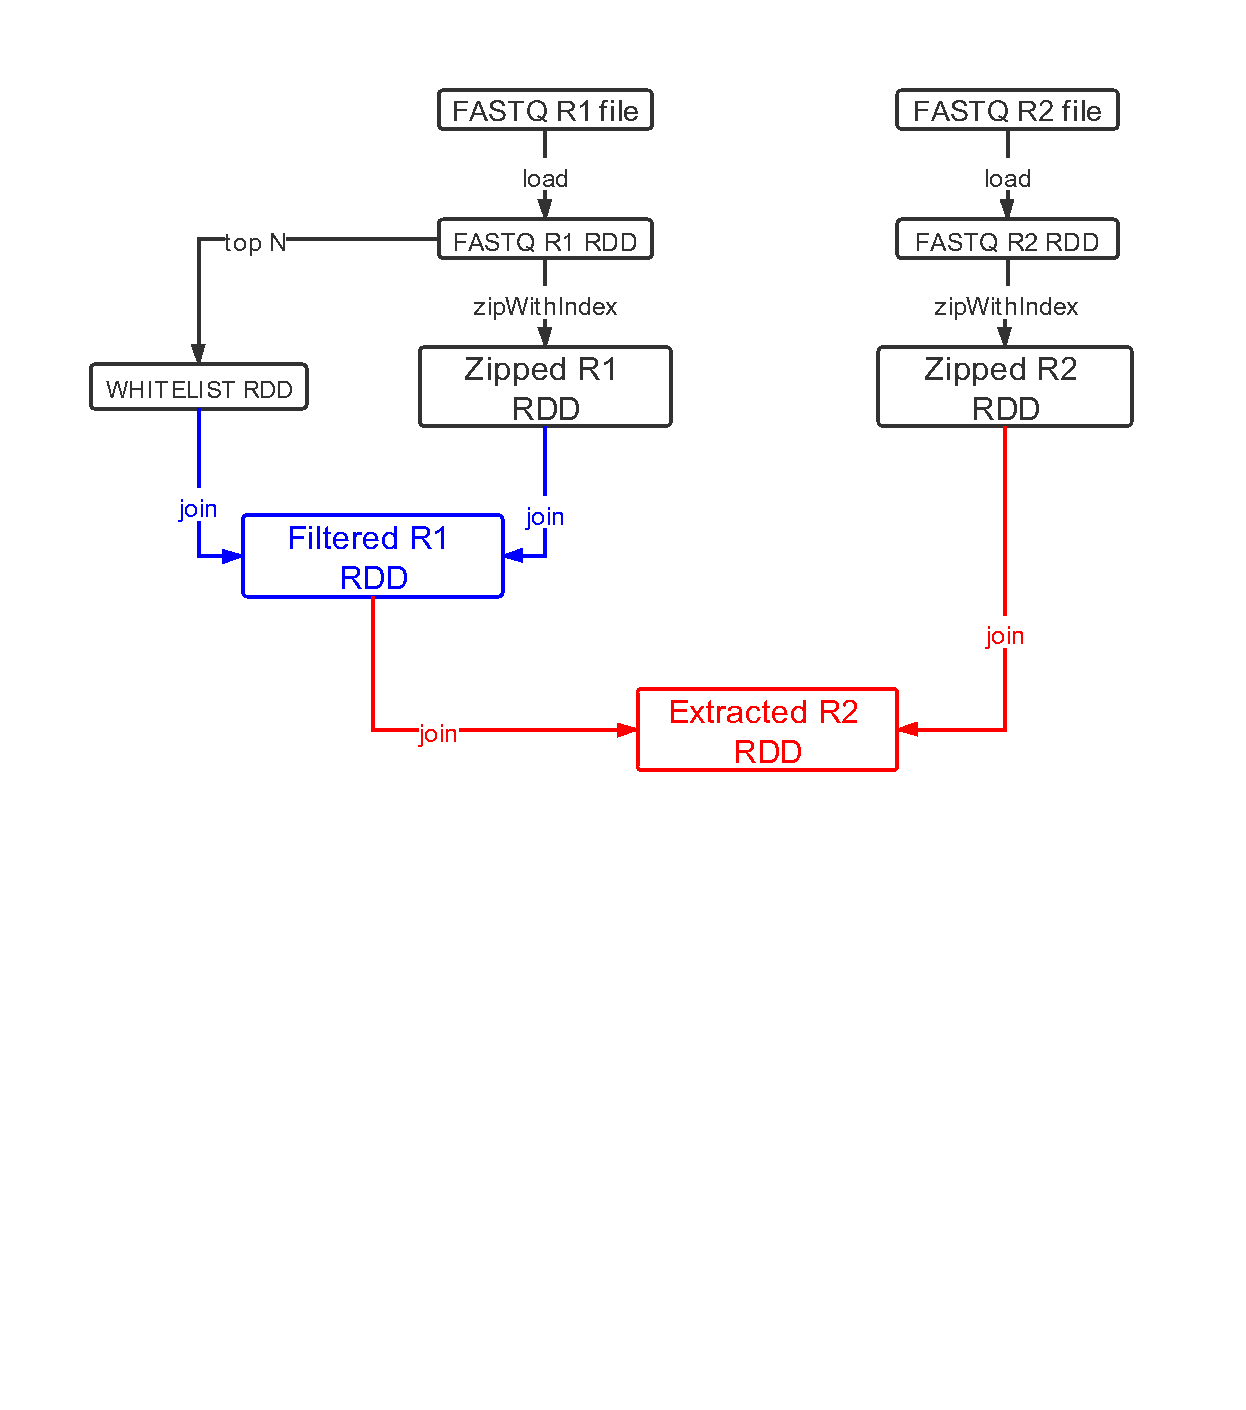
\includegraphics[width=0.98\textwidth]{fig1.pdf}
	\caption{Using JNI and RDD to integrate the STAR aligner in scSpark.} \label{fig1}
\end{figure*}

As in CellRanger, UMI-tools and STARsolo, we also adopt STAR as the aligner in scSpark.
The conventional STAR alignment procedure loads raw reads from FASTQ files and writes alignment results to Sequence Aligment/Map (SAM) or the compressed binary version of a SAM (BAM)~\cite{li2009sequence} file, requiring extensive disk access which consumes a significant amount of time.
Instead, in scSpark, we use the Java Native Interface (JNI)~(\cite{kim2012benchmarking}) to directly feed FASTQ RDD to STAR, and further transfer the results output from STAR to the SAM RDD after alignment (Fig.~\ref{fig1}.a). 
In such way, the alignment process is performed in an in-memory computing manner without any redundant disk access causes from temporyary result. 

To balance the workloads across different nodes for parallel processing, we use the Spark function \textit{repartition} before alignment to split FASTQ RDDs into \textit{N} subsets where \textit{N} denotes the number of nodes available in the cluster.
After data partitioning and shuffling, the STAR alignment is performed in parallel on all computational nodes, directly resulting in a SAM RDD which is used as an input to the next module.

\subsection{Transcript quantification}
For transcript quantification, we first use the \textit{textFile} function in Spark to load the gene transfer format (GTF)~\cite{breese2013ngsutils} file which is line structure into memory as GTF RDDs (Fig.~\ref{fig1}.b). 
After alignment, both SAM RDDs and GTF RDDs were individually grouped by chromosome into Grouped SAM RDDs and Grouped GTF RDDs respectively for parallel processing by easily using the Spark function \textit{groupByKey}. 

The gene names are then assigned to each aligned read using the \textit{join} function and user defined function. 
In scSpark, we reimplemented the directional algorithm designed by UMI-tools for transcript quantification in \textit{flatMap} function which can parallel process each cell's result in the same time. 

Finally, the resulting expression matrix can easily write upstream pipeline's result to disk or distributed file system by using default Spark's action function like \textit{saveAsTextfile} for further downstream analysis. 

\section{Results}

\subsection{Experiment design}
The performance in processing speed of scSpark is compared with CellRanger, UMI-tools and STARsolo. 
We used Apache Spark (version 2.1.0) as scSpark's in-memory computing environment. 
Three scRNA-seq datasets containing peripheral blood mononuclear cells (PBMCs) from three different species, namely human, rat and monkey, generated by 10X Genomics platform were used in our experiments. 
In total, there are approximately 640 million, 289 million and 262 million reads in the raw data of the PBMC\_human, PBMC\_rat and PBMC\_monkey datasets, respectively. 
In all the experiments, we run all the four pipelines with exactly the same cell number and barcode pattern arguments.
Pre-tests were performed to ensure sufficient memory for each pipeline.

To identify whether scSpark get better performance than three state-of-the-art pipelines in same CPU cores number condition,
we compared scSpark's performance on a cluster with 64 (16$\times$4) CPU cores with the other three pipelines' performance on a workstation with 64 CPU cores.
In this experiment, the number of CPU cores used was configured using the \textit{runThreadN} parameter for STAR and STARsolo, and the \textit{localcores} parameter for CellRanger. 
To test improvement in scSpark's performance as a result of improving each substep's performance,
we meatured UMI-tools and scSpark each substep's process time to prove scSpark get improve in any single substep.

Furthermore, to identify whether scSpark's scalability is better than three tradition pipelines, 
we meatured each tradition pipelines' speedup by considering 16 CPU cores execution as a baseline on PBMC\_human dataset.
And we used \textit{SPARK\_EXECUTOR\_CORES} parameter to restrict Spark cluster's CPU cores number, and meatured scSpark's speedup by considering 16 CPU cores execution time as a baseline on PBMC\_human dataset.
Particularly, we meatured STAR mapping's speedup by considering 16 CPU cores execution time as a baseline and meatured scSpark mapping's speedup by considering 16 CPU cores execution as a baseline on PBMC\_human dataset.
Moreover we tested scSpark's speedup and mapping speed by considering 128 CPU cores execution times as a baseline on three datasets when CPU cores number between 128 and 256 condition to prove scSpark can scale-out more efficiency than three tradition pipelines.

We also identified whether FASTQ data volume will influence scSpark's scalability.
We splited PBMC\_human dataset into 80 millions, 160 millions and 320 millions reads.
We processed PBMC\_human and three sub datasets on scSpark with different CPU cores number condition.
After that we compare each dataset's performance to evaluated whether FASTQ data volume will influence scSpark's performance.

ScSpark is developed based on UMI-tools. 
And UMI-tools accuracy was fully verified. 
This section we used the gene expression matrix that was obtained by scSpark and UMI-tools under the same dataset to perform downstream analysis of scRNA-seq data. 
And then we compared two tools transcript analysis's result and cell cluster analysis's result to verify the correlation between scSpark and UMI-tools. 
Under hgmm-10k-v3 dataset, we used scSpark and UMI-tools to get gene express matrix, compared two tools' result, and computed their correlation.


\subsection{Efficiency evaluation}

\begin{table}
	\centering
	\caption{Comparison of processing time (seconds) of four pipelines.}\label{tab1}
	\begin{tabular}{l | l | l | l }
		\hline
		 & PBMC\_human & PBMC\_rat & PBMC\_monkey \\ 
		\hline
		UMI-tools & 7284 & 7259 & 7809 \\
		CellRanger & 2225 & 1999 & 1891 \\
		STARsolo & 1987 & 1854 & 2357 \\
		\textbf{scSpark} & \textbf{355} & \textbf{326} & \textbf{391} \\
		\hline
	\end{tabular}
\end{table}

We first evaluated the total time comsumption for different pipelines processing the same dataset with the same numbers of CPUs. 
For UMI-tools, CellRanger, and STARsolo, we used all 64 cores of a single workstation. 
For scSpark, we used a cluster of 4 computing nodes, where each node has 16 CPU cores. 
Results show that scSpark achieves substantially higher processing speed, which is nearly 20-fold faster than UMI-tools and about 5-fold faster than CellRanger and STARsolo (Table~\ref{tab1}). 

\begin{figure*}
	\centering
	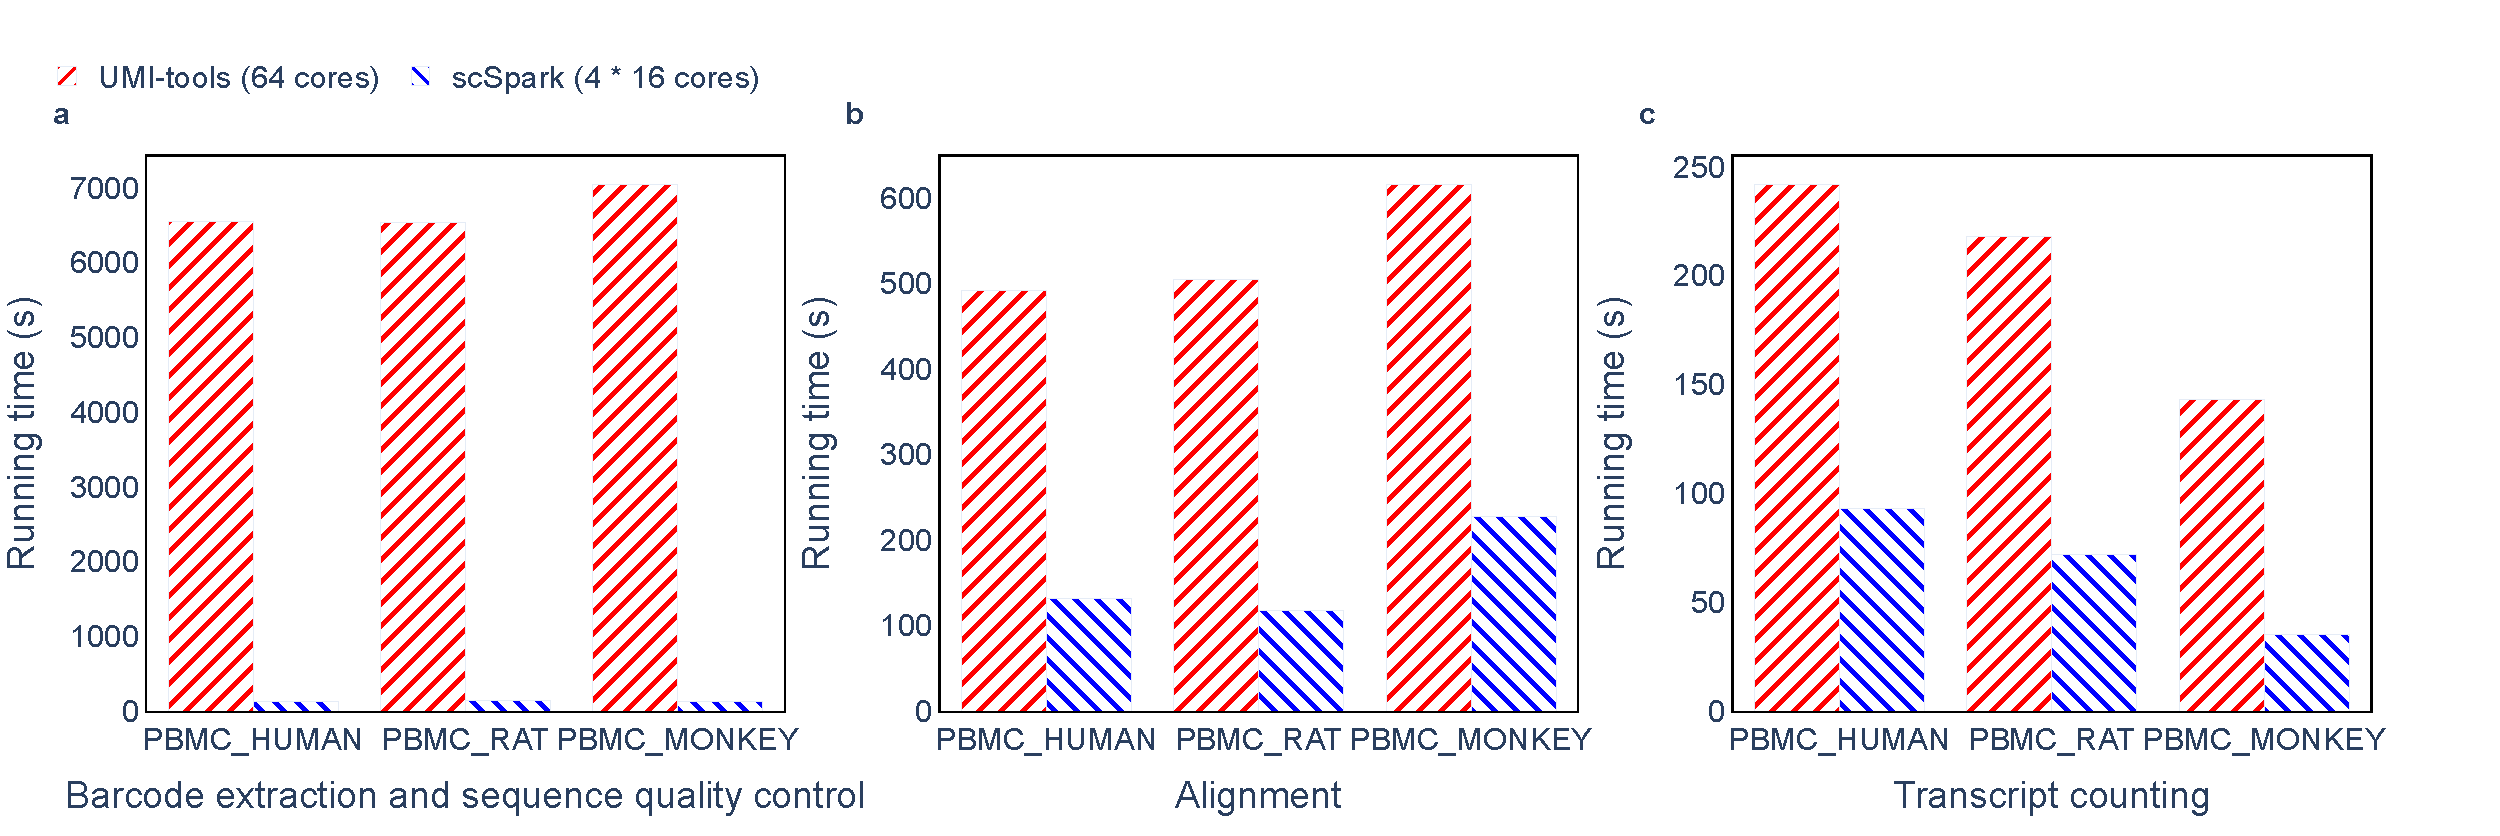
\includegraphics[width=0.98\textwidth]{fig2.pdf}
	\caption{Comparison of UMI\-tools and scSpark's first step.} \label{fig2}
\end{figure*}
We also recorded the processing time for three individual modules of the pipelines, i.e., barcode extraction and sequence QC, genome alignment, and transcript quantification, to have a more detailed understanding of the performance gain. 
As scSpark is built based on UMI-tools, the breakdown comparison was only between UMI-tools and scSpark, to demonstrate the performance gain brought by distributed and in-memory computing.
Compared with UMI-tools, scSpark had significantly shorter processing time in all three steps (Fig.~\ref{fig2}).
It is noteworthy that scSpark achieved a processsing speed of approximately 50-fold faster than UMI-tools for the barcode extraction and sequence QC step, which turned out to be the dominant factor of the performance promotion brought by scSpark.
And we found if scSpark and STAR both reduce genome load time, scSpark can get more than linear improve than STAR in align step which can prove scSpark can reduce align step's mapping time by reducing disk access.
The imporve in transcript counting step is influenced by data imbalance but its performance is more than 2-fold than UMI\-tools.

This result reflects that distributed processing of FASTQ reads from disk and totally removal of re-writing temporary results back to disk that are both performed in scSpark can dramatically reduce the time consumption of scRNA-seq data processing pipelines. 

\subsection{Evaluation of scalability} 
Contrast with tradition pipelines, scSpark not only can perform well in same CPU cores but also scSpark can scala-out to improve process speed.
\begin{figure*}
	\centering
	\subfigure[An overview of tradition pipelines' speedup.]{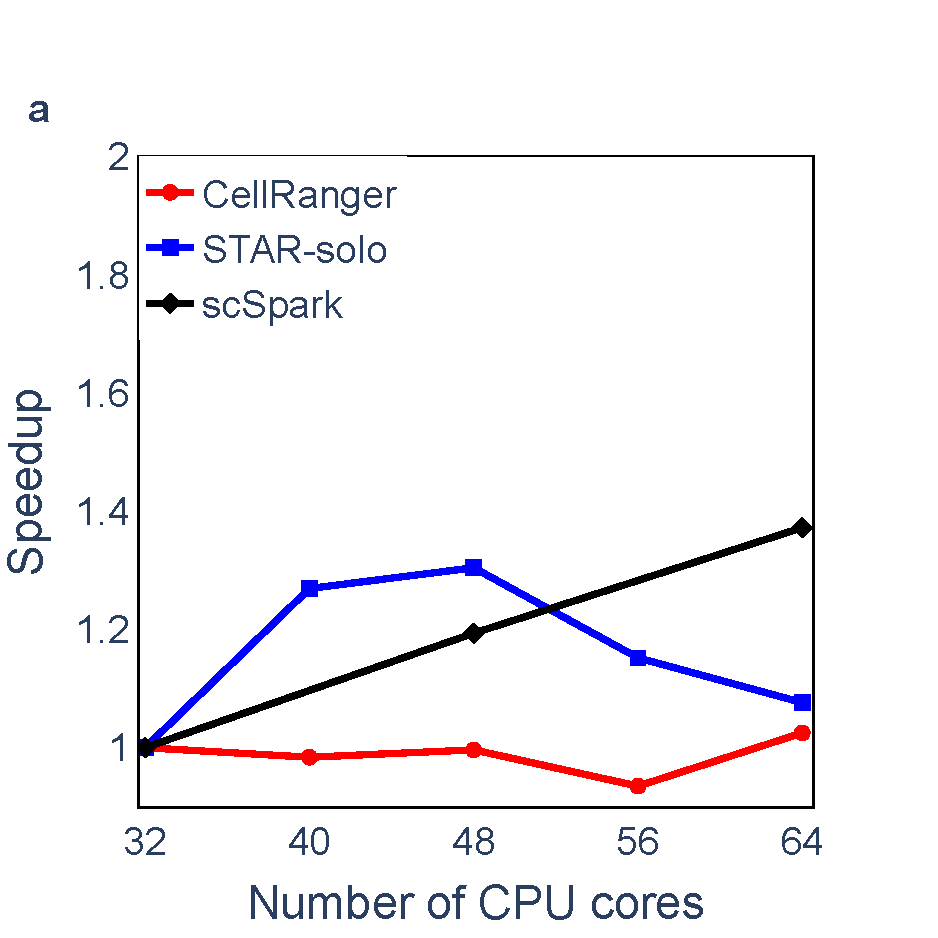
\includegraphics[width=0.48\textwidth]{fig3a.pdf}}
	\subfigure[An overview of scSpark's speedup.]{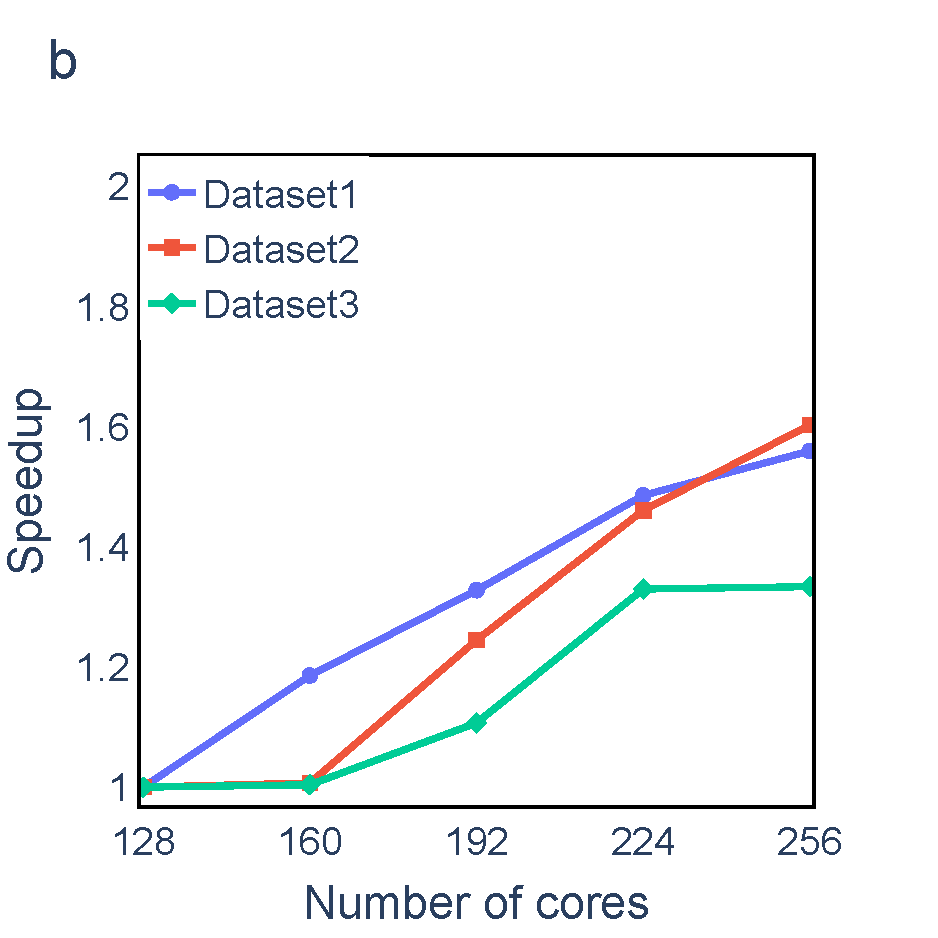
\includegraphics[width=0.48\textwidth]{fig3b.pdf}}
	\caption{ pipelines' scalability }
	\label{fig3}
\end{figure*}

Due to the limited of single workstation CPU cores, we tested STAR-solo and CellRanger's speedup from 32 CPU cores to 64 CPU cores.
And due to the limited of memory capacity per node, we tested scSpark's speedup starting from 32 (2$\times$16) CPU cores to 64 (4$\times$16) CPU cores.

As Fig~\ref{fig3}.a shown, STAR-solo's speedup can get improve under 48 CPU cores.
But when CPU cores number bigger than 48, STAR-solo's performace even weaker than the performance in 48 CPU cores condition.
This shows STAR-solo's scalability can get imporve when CPU cores number increase but STAR's performance can't scale-out with CPU cores number increase.

And we found when CPU cores number bigger than 32, CellRanger's speedup can't take advantage of CPU cores number increase.
This shows CellRanger lacks scalability when CPU cores number bigger than 32.

We found scSpark can get higher scalability than tradition pipelines when CPU cores number under 64.
Furthermore, as Fig~\ref{fig3}.b shown, scSpark achieve average 50\% speedup when Spark's CPU cores number increased from 128 to 256.

In pretest, we found that UMI\-tools' performance can't take advantage of CPU core number increase because it only be supported on single\-thread mode except align step.
Although STAR can provides scalability on align step, the whole UMI\-tools pipeline's scalability is weak.

So scSpark shows more scalability than three tradition pipelines when CPU cores number increase.

\begin{figure*}
	\centering
	\subfigure[STAR's mapping speedup contrast with scSpark's mapping speed.]{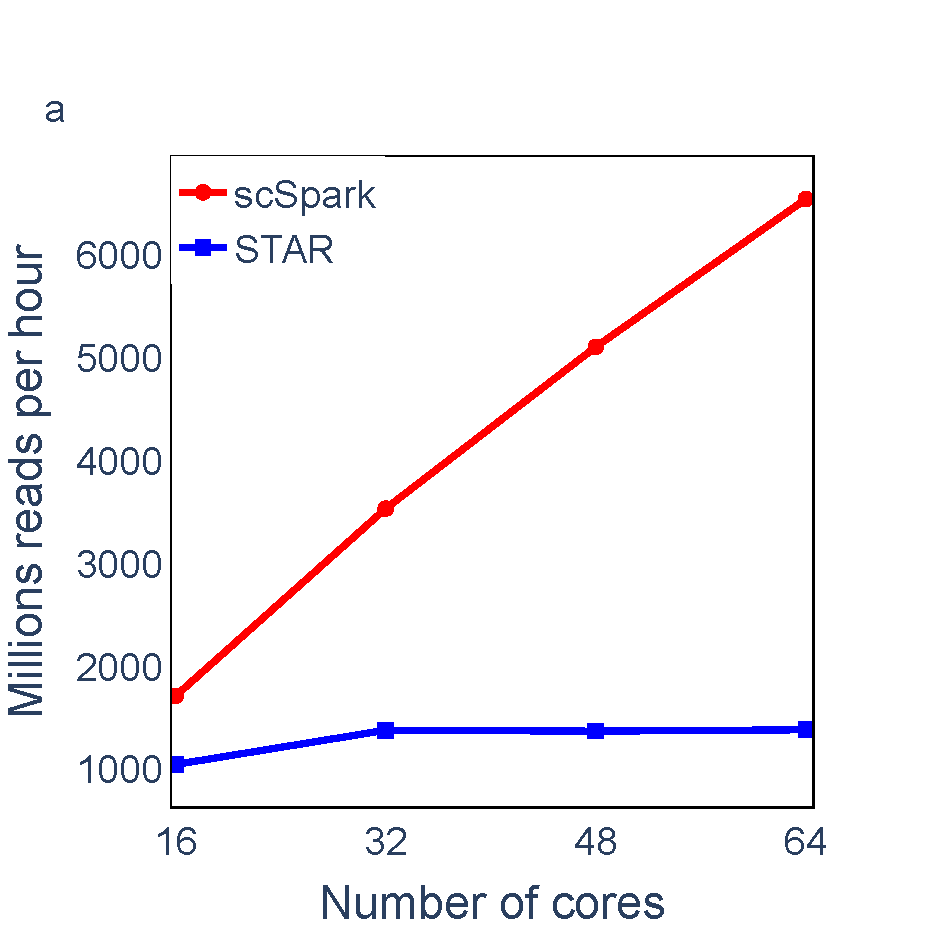
\includegraphics[width=0.48\textwidth]{fig4a.pdf}}
	\subfigure[scSpark's mapping speedup.]{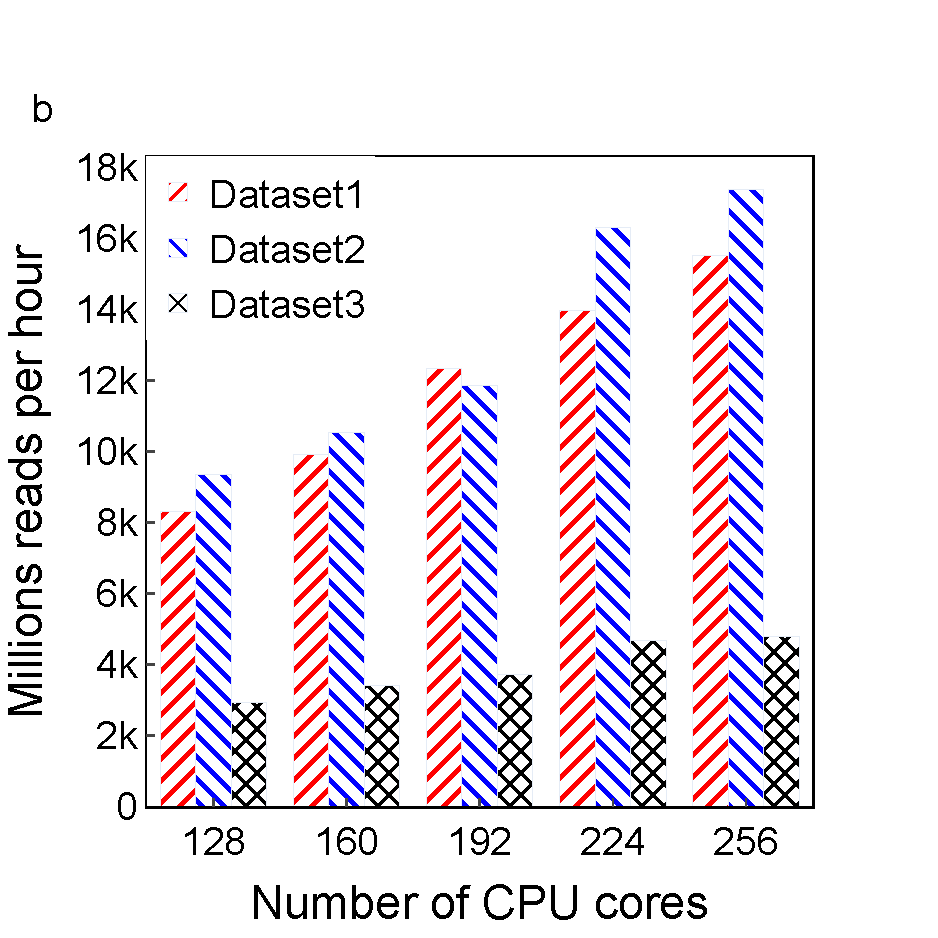
\includegraphics[width=0.48\textwidth]{fig4b.pdf}}
	\caption{ pipelines' mapping speed }
	\label{fig4}
\end{figure*}

As Fig~\ref{fig4}.a shown, we found in align step, scSpark can get much higher mapping speed than STAR in any same CPU cores number condition.
The mapping speed's imporve of scSpark not only comes from reduce disk access which conclude in last subsection but also comes from parallel compute in each node.
Furthermore, we found scSpark's mapping speed can get nearly linear parallel efficiency with CPU cores number increase.
Although STAR's mapping speed can get improve when CPU core number between 16 and 32, STAR's mapping speed improve will converage when CPU cores number bigger than 32.
And as Fig~\ref{fig4}.b shown, scSpark's mapping speed can get linear parallel efficiency even CPU cores number scale out to 256.

\subsection{Scalability influenced by data volume}
In experiment, we also found scSpark's performace influenced by data volume.

\begin{figure}
	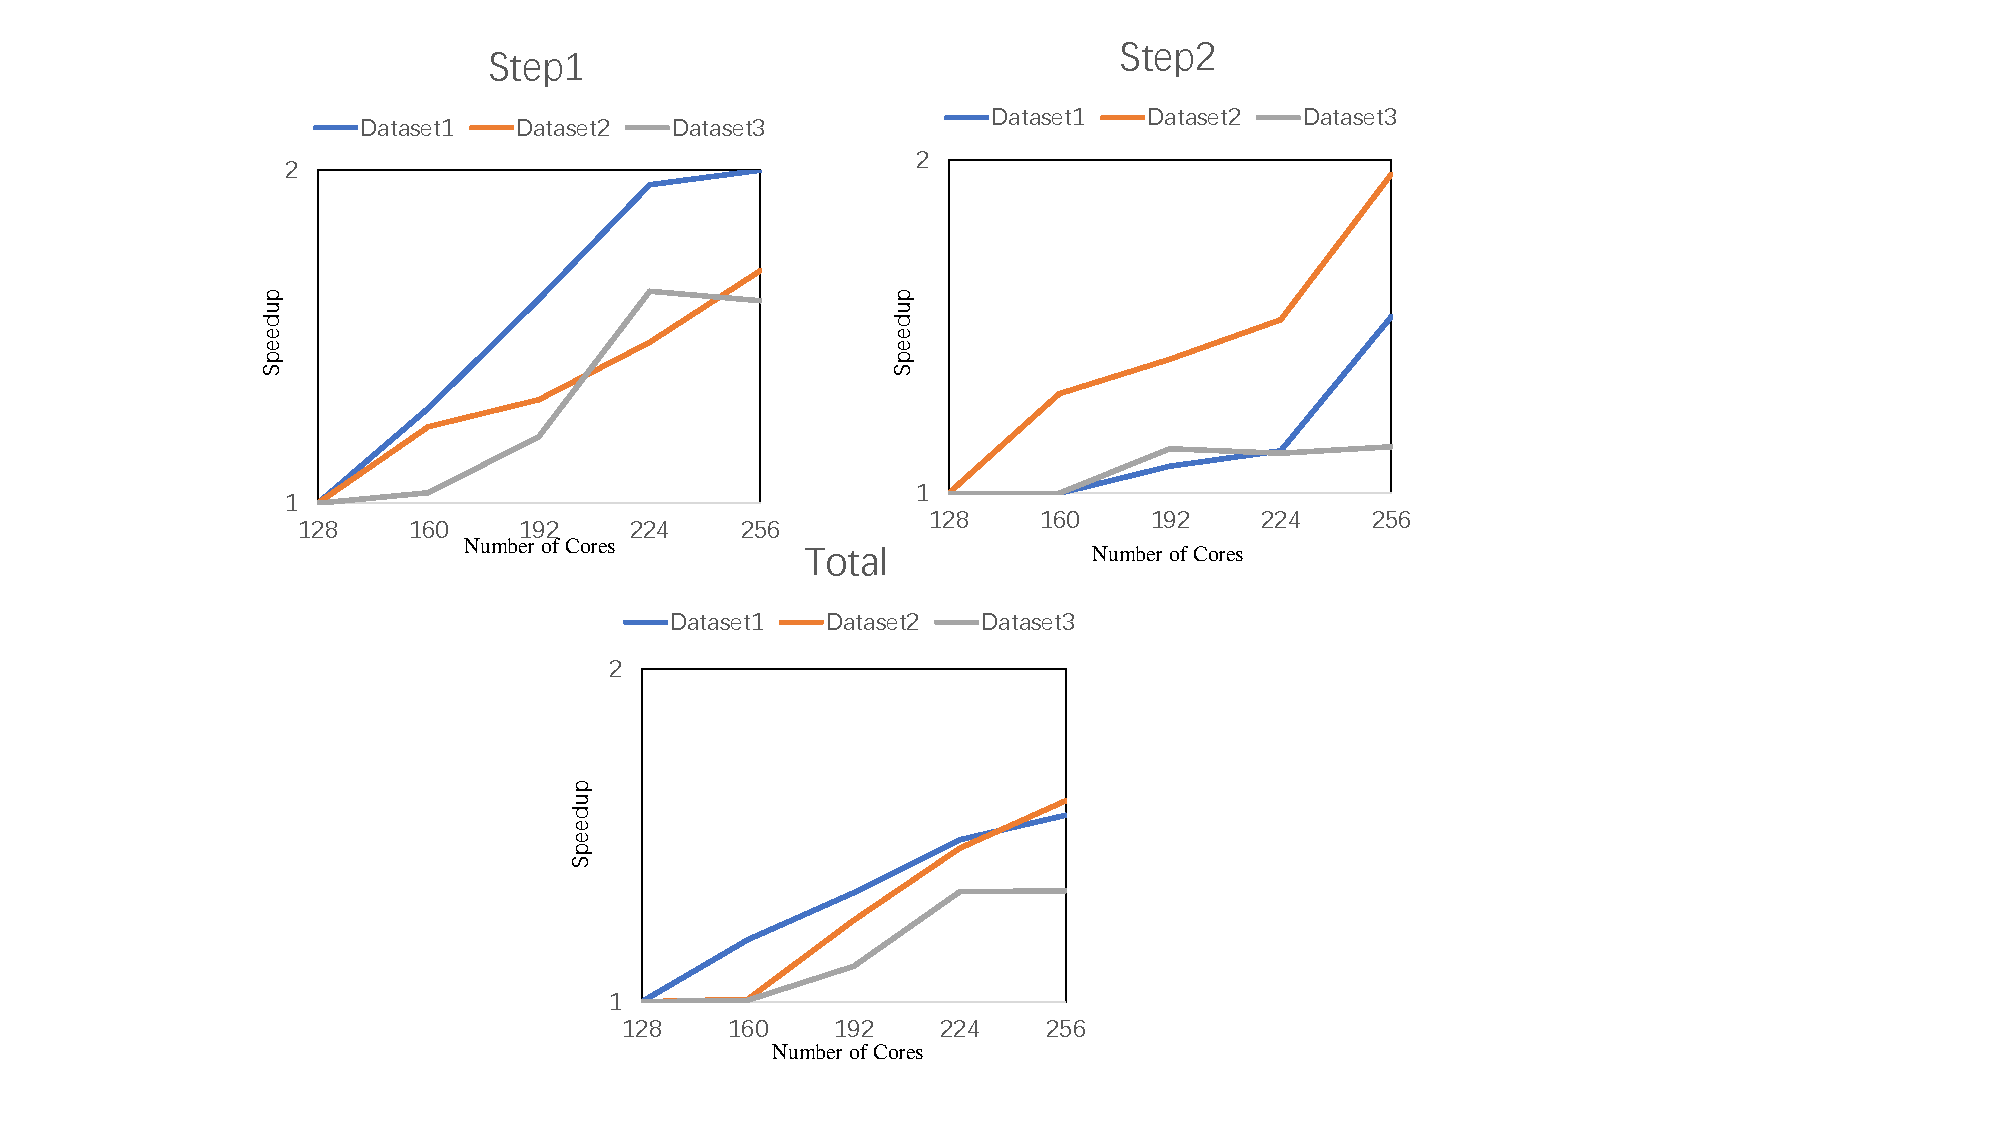
\includegraphics[width=0.48\textwidth]{fig5.pdf}
	\caption{scSpark's speedup influenced by data volume.} \label{fig5}
\end{figure}
As Fig~\ref{fig5} shown, when dataset contains 80 millions reads, scSpark's speedup is much less than dataset which contains 640 millions in CPU cores number between 128 and 256 condition.
Moreover, scSpark's speedup will converage when dataset contains 80 millions reads or 160 millions reads and CPU cores number bigger than 192.
Contrast with small dataset, scSpark's speedup can get increase when dataset contains 320 millions reads or 640 millions reads and CPU cores number bigger than 192.
So scSpark can scala-out more efficiency when scSpark processes larger dataset.

\subsection{Reliability of the results produced by scSpark} 
We further evaluated the accuracy of the expression matrices generated by scSpark.
\begin{figure}
	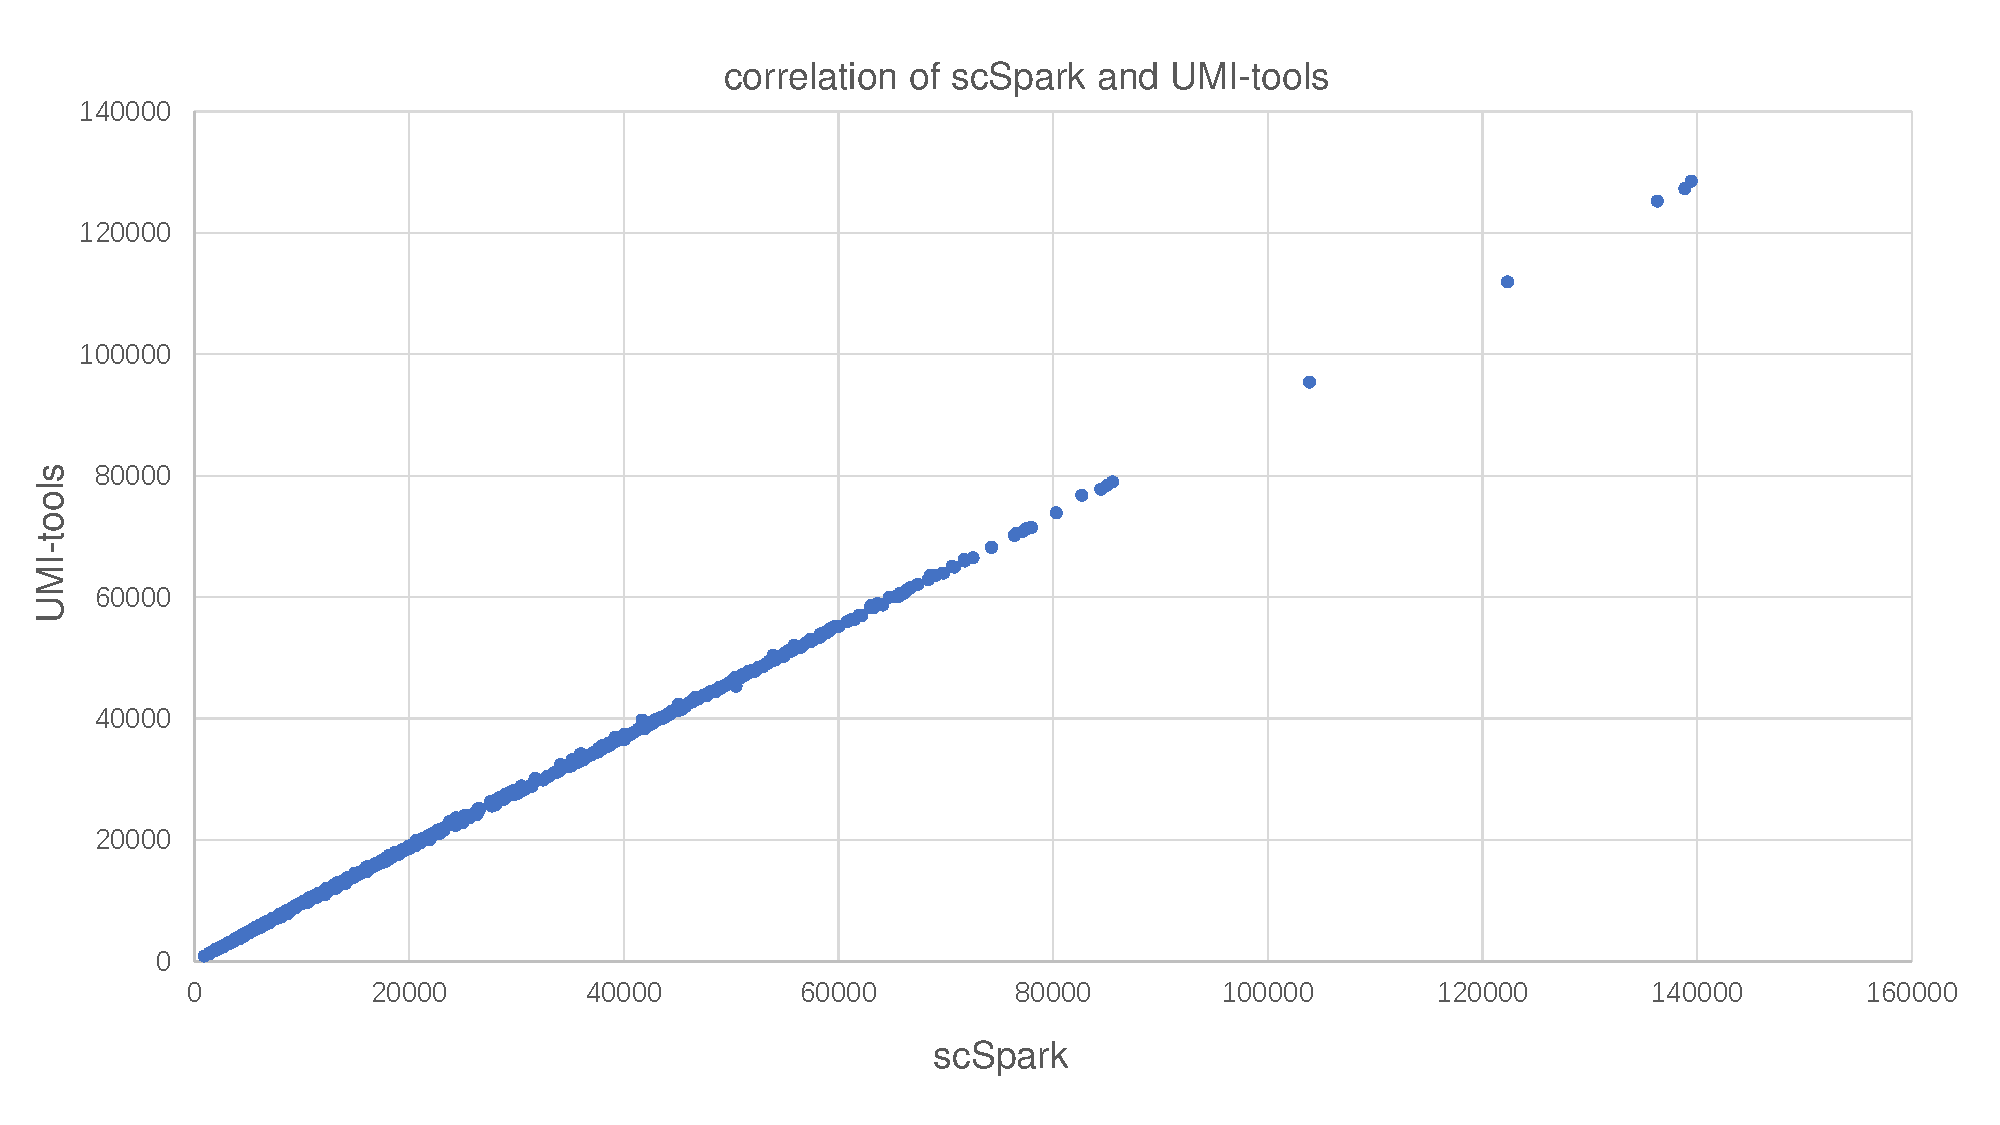
\includegraphics[width=0.48\textwidth]{fig6.pdf}
	\caption{correlation of scSpark and UMI-tools.} \label{fig8}
\end{figure}
First, the total UMI count for each cell in PBMC\_human dataset produced by scSpark was highly consistent with that by UMI-tools, with a Pearson correlation of $R^{2} = 0.9998$ (Fig~\ref{fig8}), which indicates that the expression profile of single cells produced by scSpark is reliable.
In addition, we also evaluated whether scSpark would have influence on downstream biological analysis.
Results show that the cell embeddings in tSNE map were highly consistent between scSpark and UMI-tools (Fig~\ref{fig9}).
This further demonstrates that the expression matrices generated by scSpark are accurate and would not bring interference to various types of downstream analysis such as clustering, dimension reduction and cell type identification.

\begin{figure*}
  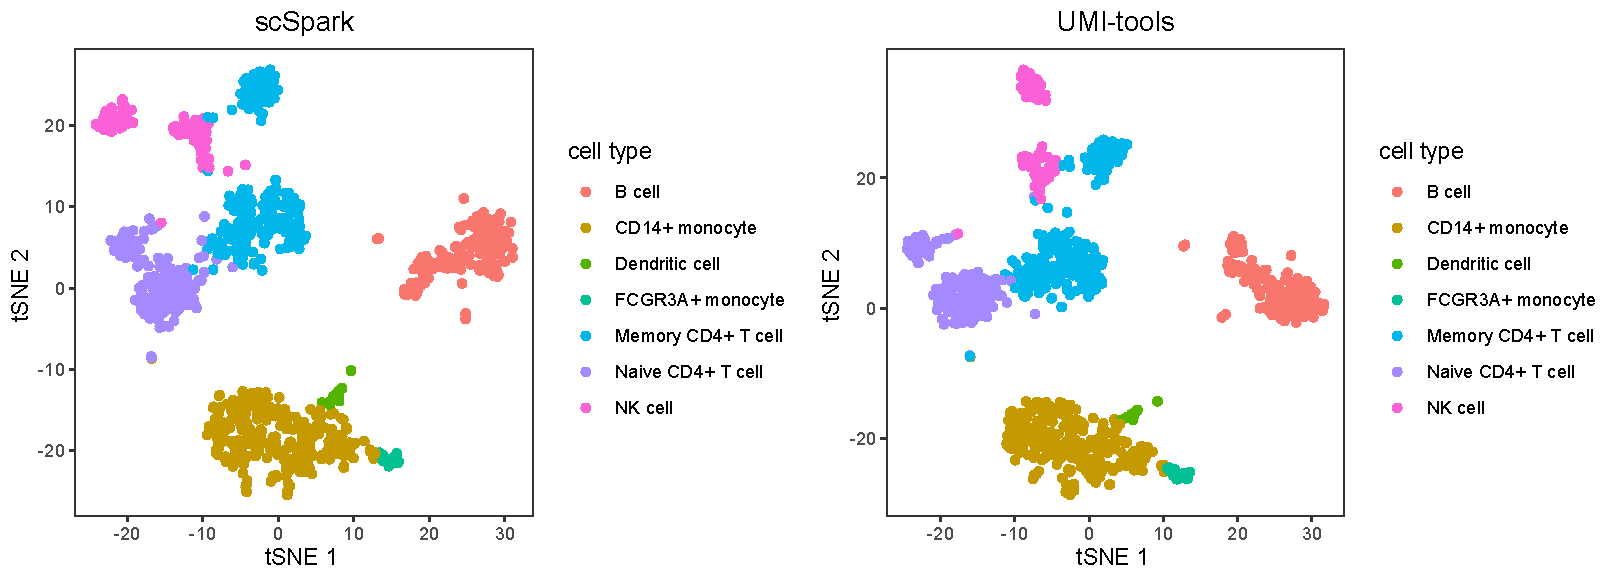
\includegraphics[width=\textwidth]{fig7.pdf}
  \caption{tSNE picture based on scSpark and UMI-tools' gene expression matrix.} \label{fig9}
\end{figure*}

\section{Conclusion}
To the volume and value of scRNA-seq data proliferated, we developed a pipeline scSpark.
ScSpark is an efficiently, highly scalable parallel compute pipeline on the top of Spark.
ScSpark not only more efficiently than tradition pipelines in same CPU cores number condition but also more scalability than tradition pipelines.
ScSpark's strategy reduce the exection time with speedup between 5 and 20 times at 64 CPU cores.
And scSpark can scale-out more than 256 CPU cores contrast with tradition pipelines' performance will converage when workstation scale-out 64 CPU cores.
Moreover, we found scSpark shows more scalability when FASTQ dataset increase.
So scSpark have potential to processed increasing FASTQ dataset by making Spark cluster bigger.
We also believe that scSpark result biological was confirmed. 

\bibliographystyle{IEEEtran}
\bibliography{reference}

\end{document}
